% LaTeX Curriculum Vitae Template
%
% Copyright (C) 2004-2009 Jason Blevins <jrblevin@sdf.lonestar.org>
% http://jblevins.org/projects/cv-template/
%
% You may use use this document as a template to create your own CV
% and you may redistribute the source code freely. No attribution is
% required in any resulting documents. I do ask that you please leave
% this notice and the above URL in the source code if you choose to
% redistribute this file.

\documentclass[letterpaper]{article}

\usepackage{hyperref}
\usepackage{geometry}

% Comment the following lines to use the default Computer Modern font
% instead of the Palatino font provided by the mathpazo package.
% Remove the 'osf' bit if you don't like the old style figures.
\usepackage[T1]{fontenc}
\usepackage[sc,osf]{mathpazo}


% email input begin
\newread\fid
\newcommand{\readfile}[1]% #1 = filename
{\bgroup
  \endlinechar=-1
  \openin\fid=#1
  \read\fid to\filetext
  \loop\ifx\empty\filetext\relax% skip over comments
    \read\fid to\filetext
  \repeat
  \closein\fid
  \global\let\filetext=\filetext
\egroup}
\readfile{/Users/hectorbahamonde/RU/Bibliografia_PoliSci/email.txt}
% email input end

% Set your name here
\def\name{Hector Bahamonde, PhD}

% Replace this with a link to your CV if you like, or set it empty
% (as in \def\footerlink{}) to remove the link in the footer:
\def\footerlink{}
% \href{http://www.hectorbahamonde.com}{www.HectorBahamonde.com}

% The following metadata will show up in the PDF properties
\hypersetup{
  colorlinks = true,
  urlcolor = blue,
  pdfauthor = {\name},
  pdfkeywords = {political science, economic development, econometrics},
  pdftitle = {\name: Curriculum Vitae},
  pdfsubject = {Curriculum Vitae},
  pdfpagemode = UseNone
}

\geometry{
  body={6.5in, 8.5in},
  left=1.0in,
  top=1.25in
}

% Customize page headers
\pagestyle{myheadings}
\markright{{\tiny \name}}
\thispagestyle{empty}

% Custom section fonts
\usepackage{sectsty}
\sectionfont{\rmfamily\mdseries\Large}
\subsectionfont{\rmfamily\mdseries\itshape\large}

% Other possible font commands include:
% \ttfamily for teletype,
% \sffamily for sans serif,
% \bfseries for bold,
% \scshape for small caps,
% \normalsize, \large, \Large, \LARGE sizes.

% Don't indent paragraphs.
\setlength\parindent{0em}

% Make lists without bullets
\renewenvironment{itemize}{
  \begin{list}{}{
    \setlength{\leftmargin}{1.5em}
  }
}{
  \end{list}
}


%%%% HERE
\usepackage{graphicx}
\usepackage{tikz}
\usepackage{tikzpagenodes}
\usetikzlibrary{calc} 

\begin{document}


\begin{tikzpicture}[remember picture,overlay]
\clip ($(current page text area.north east)!0.0001!(current page text area.south east)!0.05!(current page text area.north west)$)
  circle (2cm) node {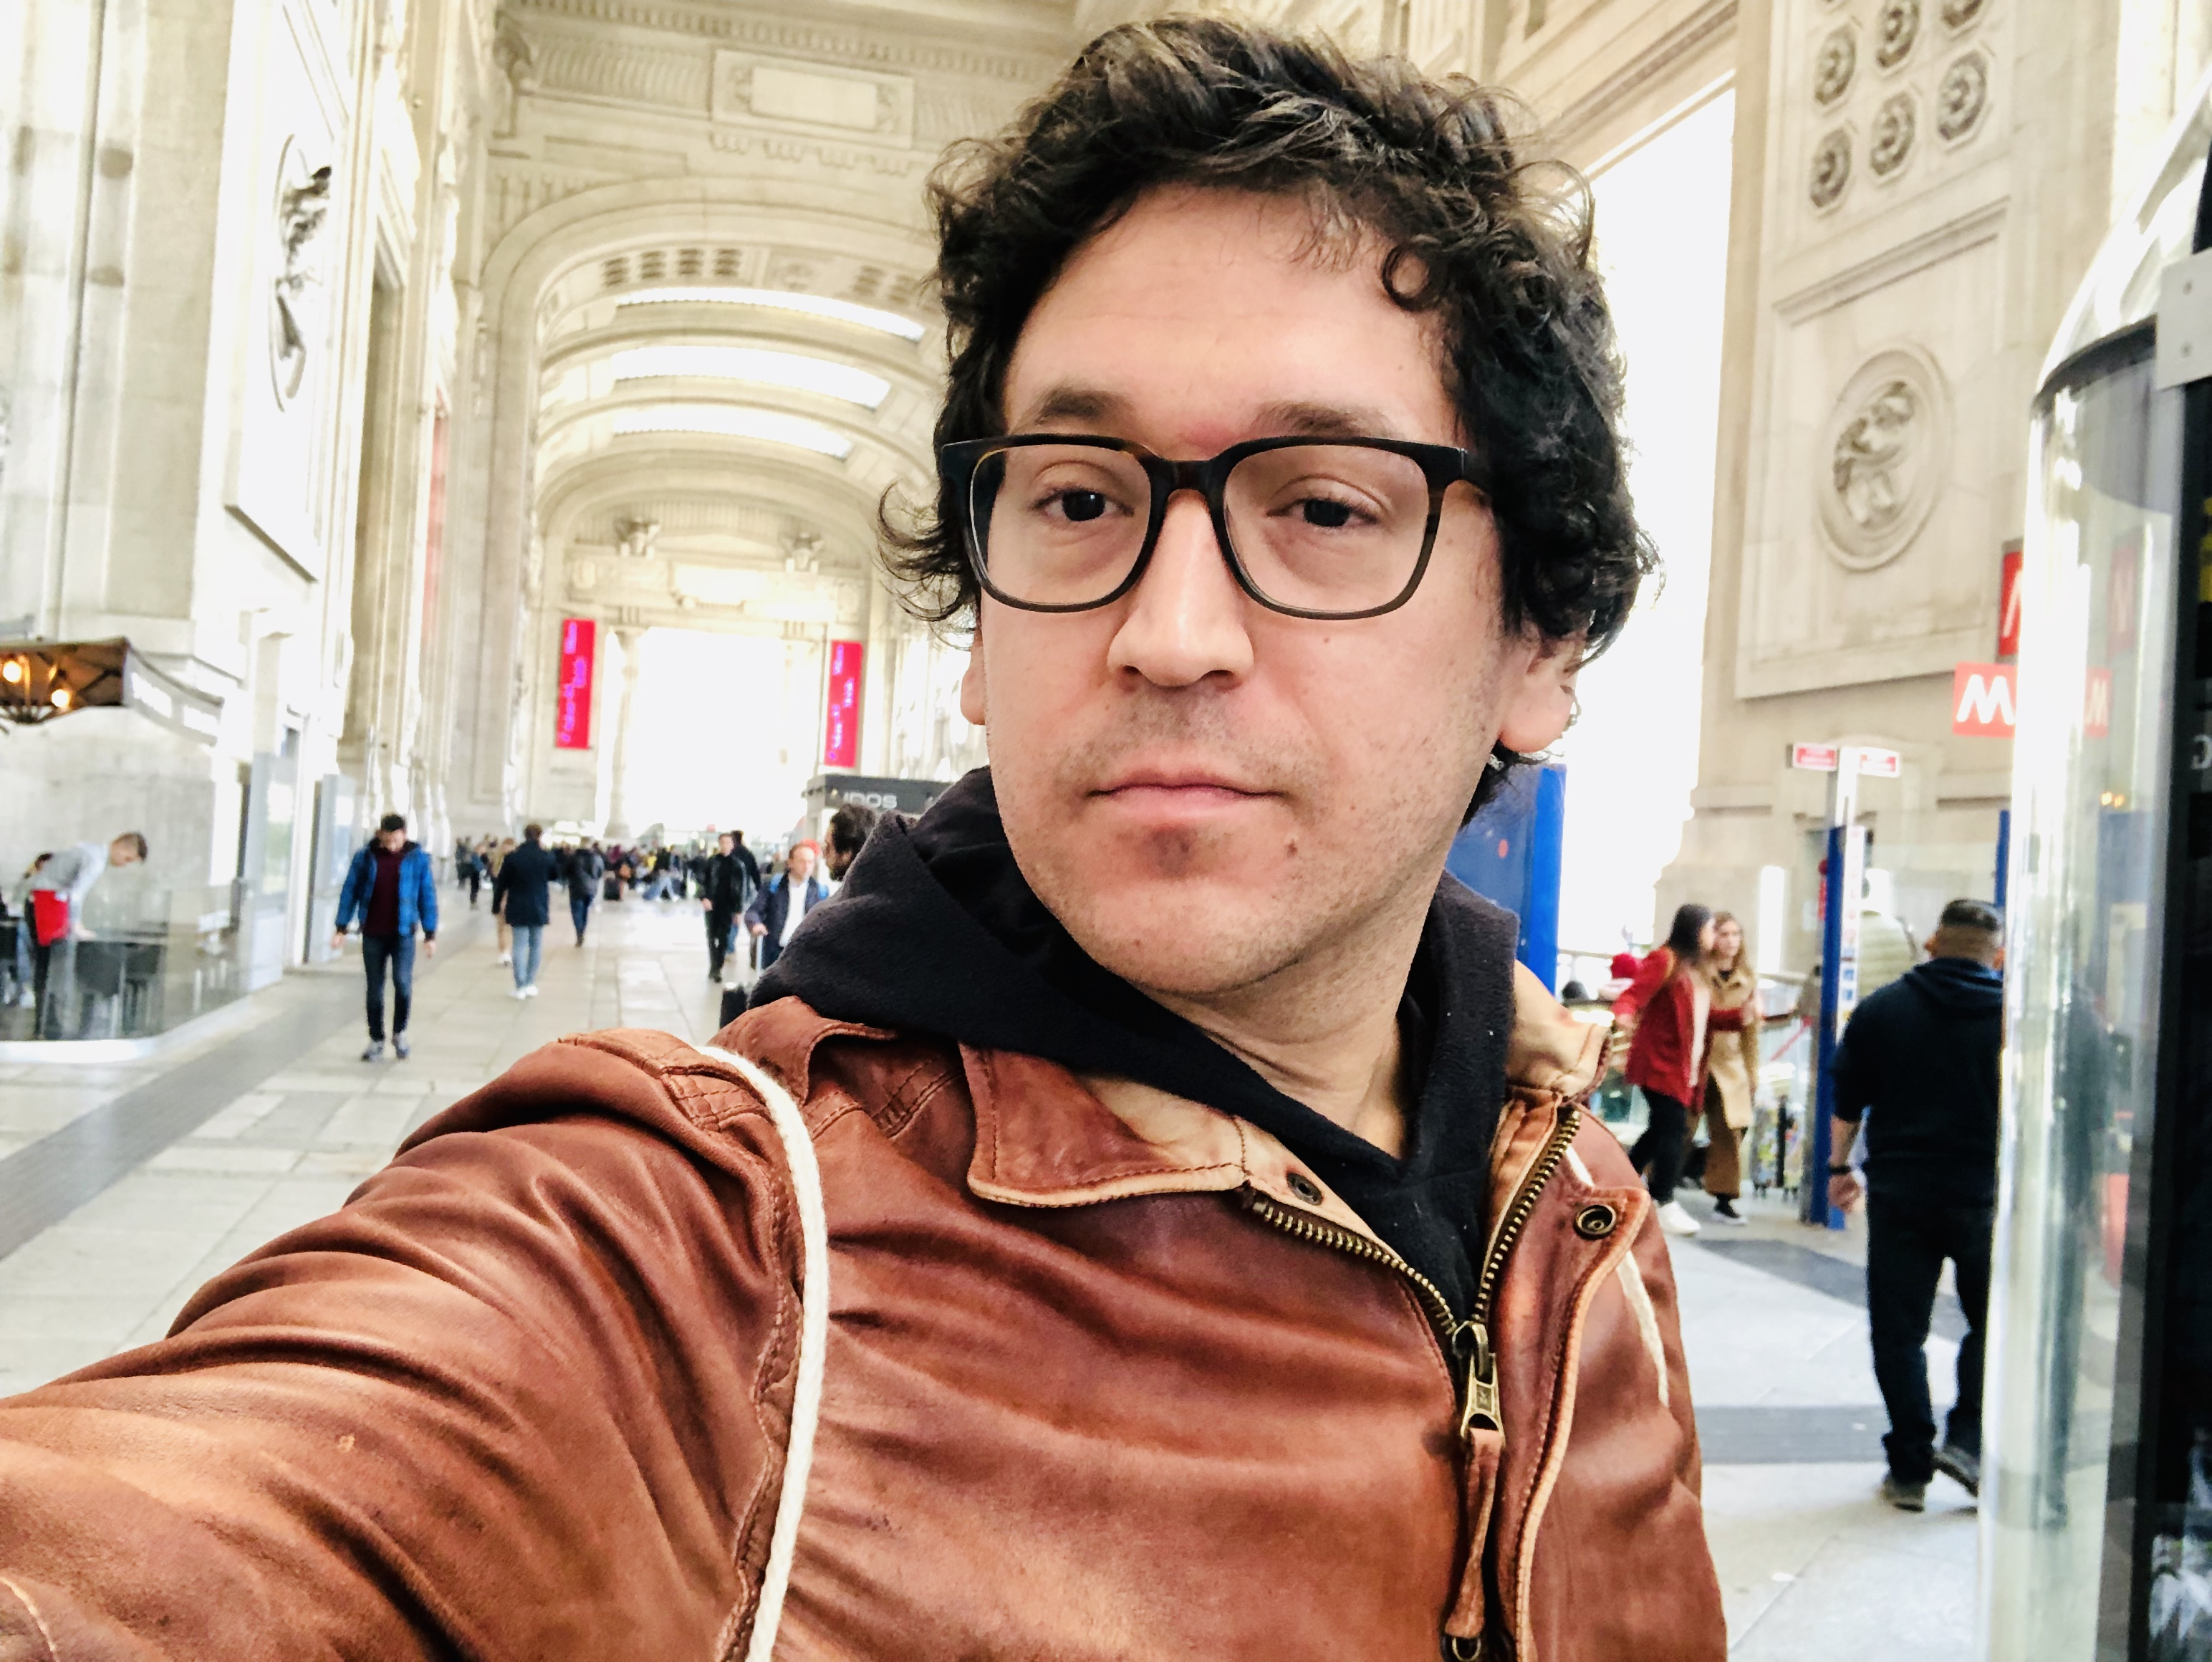
\includegraphics[width=0.2\linewidth]{profile.JPG}};
\end{tikzpicture}

\centerline{\huge \bf \name}

\vspace{0.25in}

\begin{minipage}{0.45\linewidth}
 Instituto de Ciencias Sociales \\
 Universidad de O$'$Higgins \\
 Chile\\
  \\
  \\
\begin{footnotesize}
CV last updated: \today. \\
\href{http://github.com/hbahamonde/Job_Market/raw/master/Bahamonde_NA_CV.pdf}{\texttt{{\color{red} Download latest CV here}}}.%\\
%\href{http://www.hectorbahamonde.com/jobmarket/}{\texttt{{\color{red} Download latest application materials here}}}.
\end{footnotesize}

\end{minipage}
 \hspace{\fill}\begin{minipage}{0.35\linewidth}
  \begin{tabular}{rr}
   \texttt{cp (CL)}: & +56-9-4-597-4203 \\
   \texttt{cp (US)}: & +1(504) 941-9131 \\
    \texttt{e}: & \href{mailto:\filetext}{\filetext} \\
    \texttt{w}: & \href{http://www.hectorbahamonde.com}{www.HectorBahamonde.com}\\
    \\
    \\
    \\
  \end{tabular}
\end{minipage}



%%%%%%%%%%%%%%%%%%%%%%%%%%%%%%%%%%%%%%%%%%%%%%%%%%
% Bio
%%%%%%%%%%%%%%%%%%%%%%%%%%%%%%%%%%%%%%%%%%%%%%%%%%
\section*{Bio}

Dr. Hector Bahamonde, an Assistant Professor of Political Science (political economy), has a successful academic career in Chile. In 2017 he earned his PhD in the United States. Now, being 34 years old, he's trying to relocate to Germany, get a non-academic job, and {\bf make use of his methodological training and communication-interpersonal skills outside academia}. Today, he just wants to change subjects. That is, instead of studying the most-likely \emph{voter}, he wants to learn about the most-likely \emph{consumer}/\emph{debtor}. Married to a German woman, both want to improve their work/life balance, and spend more time with Tobias (2 years-old) and Olimpia (1 year-old).



%%%%%%%%%%%%%%%%%%%%%%%%%%%%%%%%%%%%%%%%%%%%%%%%%%
% Education
%%%%%%%%%%%%%%%%%%%%%%%%%%%%%%%%%%%%%%%%%%%%%%%%%%
{\section*{Education}

\begin{itemize}
  \item {\bf Rutgers, The State University of New Jersey--New Brunswick, New Jersey, United States}\\
  Ph.D. Political Science, September 2012--May 2017.
    	\begin{itemize}
      		\item[] Dissertation: ``{\input{/Users/hectorbahamonde/RU/Dissertation/Dissertation/title.txt}\unskip}.''
      		\item[] Committee: Robert Kaufman (chair), Daniel Kelemen, Douglas Blair (Economics), Paul Poast (University of Chicago).
          \item[] {\bf Fields}: Comparative Politics and Quantitative Methodology.
		  \end{itemize}

\item {\bf Catholic University of Chile--Santiago}.\\
B.A. Political Science, 2005--2009.
\end{itemize}
\unskip}

%%%%%%%%%%%%%%%%%%%%%%%%%%%%%%%%%%%%%%%%%%%%%%%%%%
% Academic Employment
%%%%%%%%%%%%%%%%%%%%%%%%%%%%%%%%%%%%%%%%%%%%%%%%%%
\section*{Employment}

{\begin{itemize}
  \item[] {\bf Tulane University, New Orleans, LA, United States}\\
  Post-Doctoral Fellow, Center for Inter-American Policy \& Research (CIPR), 2017-present

  \item[] {\bf Rutgers University, New Brunswick, NJ, United States}\\
  Teaching Assistant, 2014-2017
\end{itemize}
\unskip}



%%%%%%%%%%%%%%%%%%%%%%%%%%%%%%%%%%%%%%%%%%%%%%%%%%
% Expertise/Interests
%%%%%%%%%%%%%%%%%%%%%%%%%%%%%%%%%%%%%%%%%%%%%%%%%%
\section*{Skills}


\subsection*{Certified Methods Proficiency}

I have graduate-level statistics training in forecasting, vector auto-regression and error correction models, Bayesian analyses, survey, laboratory and quasi experiments, linear and generalized statistical models, regression discontinuity and diff-in-diff designs. These certifications were obtained at the {\bf University of Michigan} (Ann Arbor), {\bf Princeton} and {\bf Rutgers} University (Statistics Msc programme). Below, I detail some of the courses I've taken:

\begin{itemize}
	\item[-] {\bf Forecasting}: ``Time Series,'' ``Advanced Time Series.''
	\item[-] {\bf Bayesian}: ``Introduction to Bayesian Analysis.'' 
	\item[-] {\bf Lineal Models}: ``Advanced Ordinary Least Square Methods,'' ``Regression Analysis.''
	\item[-] {\bf Non-lineal Models}: ``Advanced Maximum Likelihood-Estimation'' and ``Panel Data Analyses.''
	\item[-] {\bf Game Theory}: ``Introduction to Game Theory'' and ``Formal Modeling.''
	\item[-] {\bf Experimental Methods}: ``Experimental Methods,'' ``Causal Inference for the Social Sciences.''
\end{itemize}


\subsection*{Data-Oriented and Computational Social Scientist}
My goal is to help you making data-informed decisions. 
I'm passionate about working with big datasets, designing and implementing metrics, building statistical models to learn about customer behavior, product usage, and communicating meaningful reports. You can check my modeling expertise in my \href{https://github.com/hbahamonde}{GitHub}. Teaching and presenting at conferences are my daily routine; I'm passionate about communicating results effectively too.







\subsection*{Interpersonal}
I have considerable experience as an independent critical person, used to work under pressure, and goal-oriented. Not only do I have good writing/analytical skills, but also excellent interpersonal relationships. Having both excellent leadership skills and willingness to collaborate with others, make me an ideal candidate to take different roles, for instance in different projects, in the same institution. 





\subsection*{Others}
\begin{itemize}
	\item- {\bf Languages}: English, Spanish.
	\item- {\bf Advanced Software Usage}: \texttt{R}, \texttt{Stata}, \LaTeX.
\end{itemize}


%%%%%%%%%%%%%%%%%%%%%%%%%%%%%%%%%%%%%%%%%%%%%%%%%%
% Working Papers -- Published Papers
%%%%%%%%%%%%%%%%%%%%%%%%%%%%%%%%%%%%%%%%%%%%%%%%%%
\section*{Research}

{\bf Please note, every paper employs different sophisticated---still \emph{applied}---econometric techniques.}

{%%%%%%%%%%%%%%%%%%%%
% Working Papers
%%%%%%%%%%%%%%%%%%%%
\subsection*{Peer-Reviewed Articles}


\begin{itemize}

	\item[\textcolor{gray}{\textbullet}] \input{/Users/hectorbahamonde/research/Vote_Selling/status.txt}\unskip

	\item[\textcolor{gray}{\textbullet}] \href{https://doi.org/10.1111/rsp3.12337}{Employment Effects of Covid‐19 across Chilean Regions: An Application of the Translog Cost Function}. \emph{Regional Science, Policy and Practice}, 12: 1151---1167. With Felix Modrego and Andrea Canales.

	\item[\textcolor{gray}{\textbullet}] \input{/Users/hectorbahamonde/research/Clientelism_paper/status.txt}\unskip

	\item[\textcolor{gray}{\textbullet}] \href{https://scielo.conicyt.cl/pdf/revcipol/v31n2/art07.pdf}{El Secreto de mi \'Exito: Parte II. Los Caminos a Valpara\'iso en 2009}. \emph{Revista de Ciencia Pol\'itica}, 31(2), pp. 285---310. With Pilar Giannini, Juan Pablo Luna, Rodolfo L\'opez, Mart\'in Ordo\~nez and Gonzalo Recart.
  
\end{itemize}



\subsection*{Work in Progress}


\begin{itemize}

  	\item[\textcolor{gray}{\textbullet}] \href{https://github.com/hbahamonde/Inequality_State_Capacities/raw/master/Bahamonde_Trasberg.pdf}{\input{/Users/hectorbahamonde/research/Inequality_State_Capacities/title.txt}\unskip}, {\bf \emph{\input{/Users/hectorbahamonde/research/Inequality_State_Capacities/status.txt}\unskip}}. With Mart Trasberg (Tulane University).

	\item[\textcolor{gray}{\textbullet}] \href{https://github.com/hbahamonde/Conjoint_US/raw/master/Bahamonde_Quininao_Conjoint.pdf}{\input{/Users/hectorbahamonde/research/Conjoint_US/title.txt}\unskip}, {\bf \emph{\input{/Users/hectorbahamonde/research/Conjoint_US/status.txt}\unskip}}. With Crist\'obal Qui\~ninao (UOH).

  	\item[\textcolor{gray}{\textbullet}] \href{https://raw.githubusercontent.com/hbahamonde/Economic_Experiment_Vote_Selling/master/abstract.txt}{\input{/Users/hectorbahamonde/research/Economic_Experiment_Vote_Selling/title.txt}\unskip}, {\bf \emph{\input{/Users/hectorbahamonde/research/Economic_Experiment_Vote_Selling/status.txt}\unskip}}. With Andrea Canales.


	\item[\textcolor{gray}{\textbullet}] \href{https://raw.githubusercontent.com/hbahamonde/Tobalaba/master/abstract.txt}{\input{/Users/hectorbahamonde/research/Tobalaba/title.txt}\unskip}, {\bf \emph{\input{/Users/hectorbahamonde/research/Tobalaba/status.txt}\unskip}}. With Paz Irarrazabal.

	\item[\textcolor{gray}{\textbullet}] \href{https://www.hectorbahamonde.com}{\input{/Users/hectorbahamonde/research/Bahamonde_Kovac/title.txt}\unskip}, {\bf \emph{\input{/Users/hectorbahamonde/research/Bahamonde_Kovac/status.txt}\unskip}}. With Igor Kovac (U Cincinnati).


  	\item[\textcolor{gray}{\textbullet}]  \href{https://github.com/hbahamonde/Earthquake_Paper/raw/master/Bahamonde_Earthquake_Paper.pdf}{\input{/Users/hectorbahamonde/Dissertation/Papers/Earthquake_Paper/title.txt}\unskip}, {\bf \emph{\input{/Users/hectorbahamonde/Dissertation/Papers/Earthquake_Paper/status.txt}\unskip}}.

	\item[\textcolor{gray}{\textbullet}] \href{https://raw.githubusercontent.com/hbahamonde/IncomeTaxAdoption/master/abstract.txt}{\input{/Users/hectorbahamonde/Dissertation/Papers/IncomeTaxAdoption/title.txt}\unskip}, {\bf \emph{\input{/Users/hectorbahamonde/Dissertation/Papers/IncomeTaxAdoption/status.txt}\unskip}}.
  
  	\item[\textcolor{gray}{\textbullet}] \href{https://raw.githubusercontent.com/hbahamonde/Negative_Link_Paper/master/abstract.txt}{\input{/Users/hectorbahamonde/Dissertation/Papers/NegativeLink/title.txt}\unskip}, {\bf \emph{\input{/Users/hectorbahamonde/Dissertation/Papers/NegativeLink/status.txt}\unskip}}. 

  	\item[\textcolor{gray}{\textbullet}] \href{https://raw.githubusercontent.com/hbahamonde/Running_Tally/master/abstract.txt}{\input{/Users/hectorbahamonde/research/Running_Tally/title.txt}\unskip}, {\bf \emph{\input{/Users/hectorbahamonde/research/Running_Tally/status.txt}\unskip}}. With Richard Lau (Rutgers) and Mona Kleinberg (UMass - Lowell). 






\end{itemize}


%%%%%%%%%%%%%%%%%%%%
% Other Publications
%%%%%%%%%%%%%%%%%%%%


\subsection*{Book Reviews in Peer-Reviewed Journals (Invited)}

\begin{itemize}
	\item[\textcolor{gray}{\textbullet}] In\'es Dur\'an Matute (2019). \href{https://doi.org/10.1080/13260219.2019.1671679}{``Indigenous Peoples and the Geographies of Power: Mezcala's Narratives of Neoliberal Governance''} (Routledge). \emph{Journal of Iberian and Latin American Research}. % Scopus
\end{itemize}

\subsection*{Book Chapters}

\begin{itemize}
\item[\textcolor{gray}{\textbullet}] \href{http://www.vanderbilt.edu/lapop/chile/Chile-2010-cultura-politica.pdf}{?`Estable Pero Sin Ra\'ices? Los Partidos Pol\'iticos Chilenos en la Opini\'on P\'ublica}, in \emph{Cultura Pol\'itica de la Democracia en Chile, Ch. IX, LAPOP Country Report, 2010}. With Juan Pablo Luna, Germ\'an Bidegain, Roody Reserve and Giancarlo Visconti.
\end{itemize}



}



%%%%%%%%%%%%%%%%%%%%%%%%%%%%%%%%%%%%%%%%%%%%%%%%%%
% Career Objective
%%%%%%%%%%%%%%%%%%%%%%%%%%%%%%%%%%%%%%%%%%%%%%%%%%
\section*{Career Objective}

I want to help institutions (big or small) to reach their goals by incorporating my academic experience. By bringing my analytical skills, and excellent interpersonal relationships, I am interested in both leading teams and collaborating with others. My ideal institution lets its employees be innovative, goal-oriented and creative. {\bf I have immediate availability, and I'm ready to relocate \emph{tomorrow}.}

\section*{Personal}

Art, creativity, and others forms of self-expression, are part of who I am. I have a deep appreciation for music, photography, poetry, cinema, among others. Even cooking can be considered a way of self-expression.  I think it's important to cultivate these aspects: they make a better professional and dad. When I'm not working, I enjoy playing the bass guitar, cooking, or reading. Running and swimming are also part of my daily routine.

\bigskip



\end{document}
